\documentclass{article}
\usepackage[T1]{fontenc}
\usepackage{lmodern}
\usepackage{graphicx}
\usepackage{amsmath,amssymb}
\usepackage[a4paper,margin=2cm]{geometry}
\usepackage[absolute,overlay]{textpos}
\setlength{\TPHorizModule}{1mm}
\setlength{\TPVertModule}{1mm}
\usepackage[indonesian]{babel}
\usepackage{hyperref}
\setlength{\emergencystretch}{2em}
% unit: Halaman 28

\begin{document}

% === Halaman 28 (llm) ===

\vspace{246.51mm}

\section*{Satu putaran di dalam jaringan Feistel secara lengkap:}

\vspace{100mm}

Sumber: Cryptography and Network Security \\
Chapter 3, Lecture slides by Lawrie Brown \\
Modified by Richard Newman

% deskripsi: Diagram blok tingkat tinggi dari satu putaran jaringan Feistel yang menunjukkan operasi XOR dan fungsi f.
% bbox normalisasi: [0.7090, 0.0000, 0.9960, 0.2300]
\begin{textblock*}{60.27mm}(148.89mm,0.00mm)
\noindent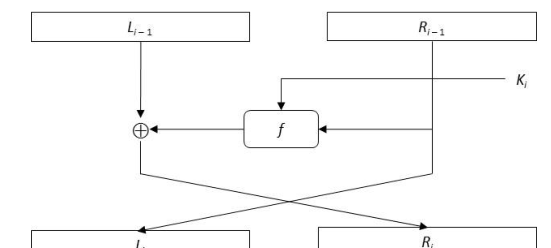
\includegraphics[width=60.27mm,height=68.31mm]{../../images/llm/page_028_img_01.png}%
\end{textblock*}

% deskripsi: Diagram alur mendetail dari satu putaran jaringan Feistel, menunjukkan permutasi bit, input simbol, S-box (S1-S8), dan ekspansi bit.
% bbox normalisasi: [0.0000, 0.1300, 0.9960, 0.9600]
\begin{textblock*}{209.16mm}(0.00mm,38.61mm)
\noindent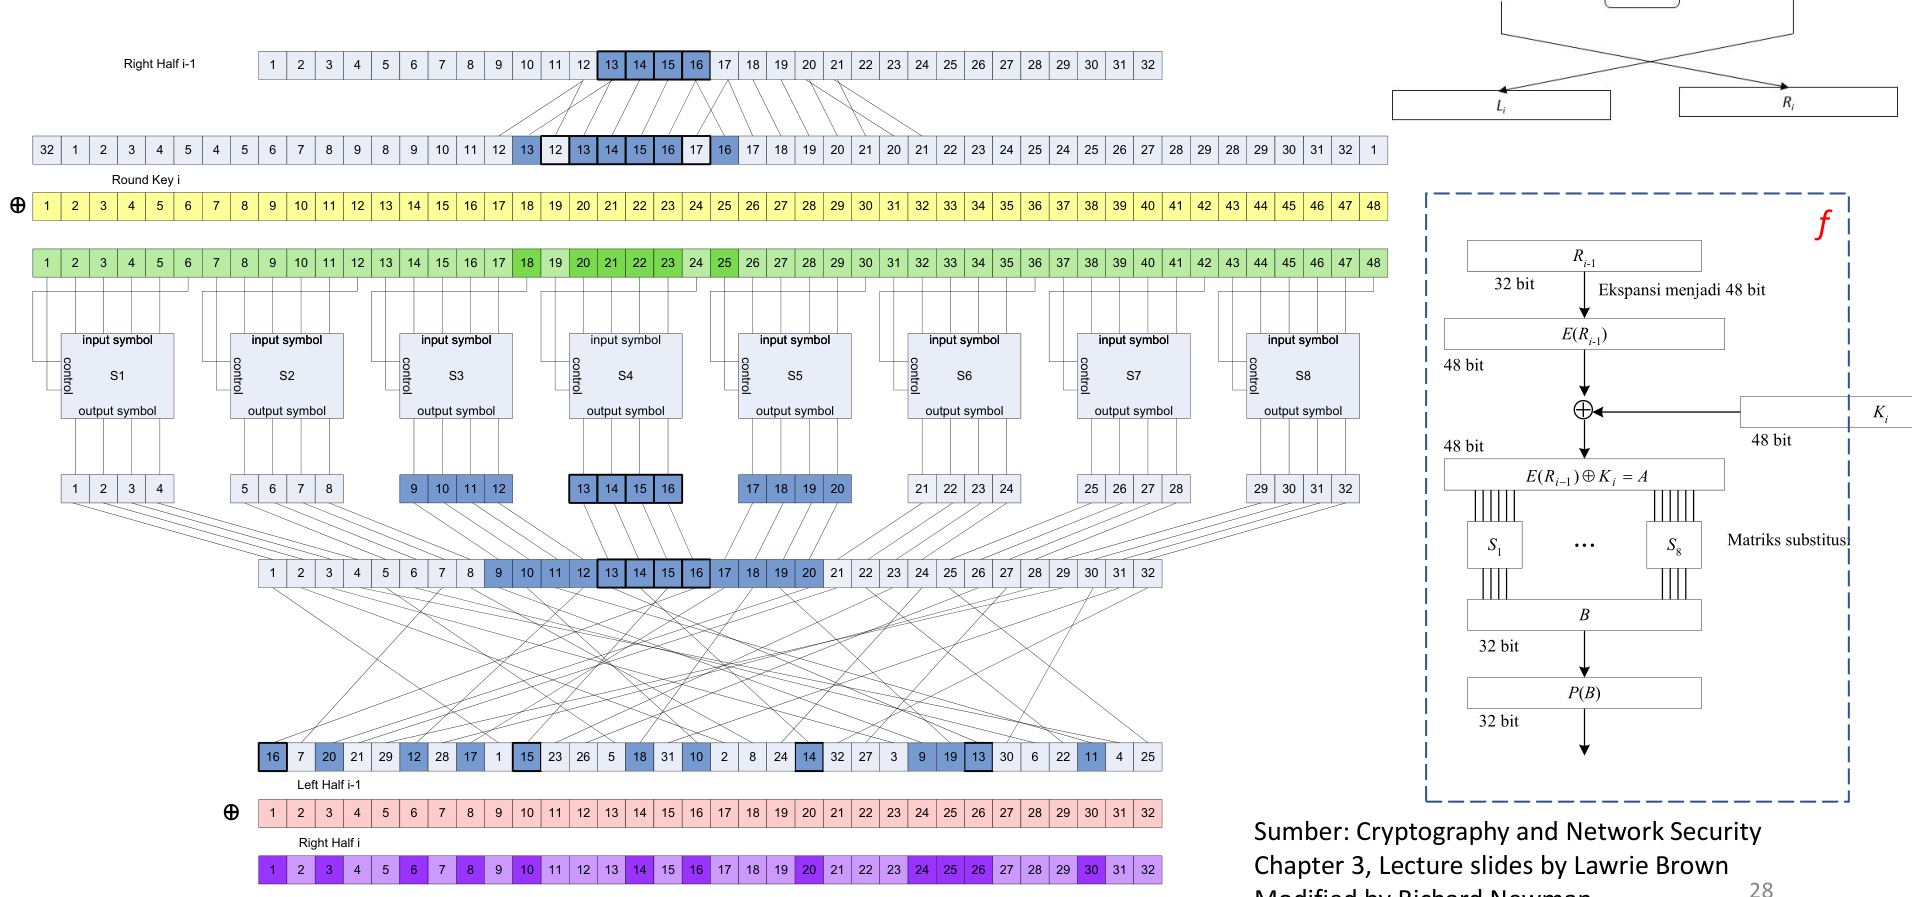
\includegraphics[width=209.16mm,height=246.51mm]{../../images/llm/page_028_img_02.png}%
\end{textblock*}

% deskripsi: Diagram detail internal fungsi f dalam jaringan Feistel, menunjukkan ekspansi, operasi XOR dengan kunci Ki, matriks substitusi S-box, dan permutasi P.
% bbox normalisasi: [0.7130, 0.2800, 0.9960, 0.8300]
\begin{textblock*}{59.43mm}(149.73mm,83.16mm)
\noindent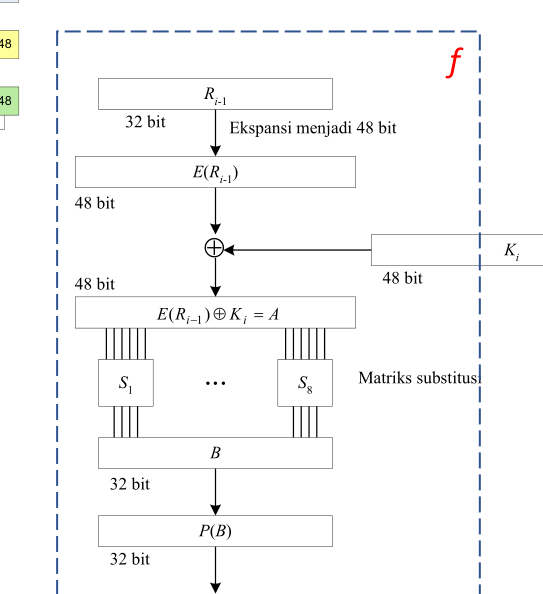
\includegraphics[width=59.43mm,height=163.35mm]{../../images/llm/page_028_img_03.png}%
\end{textblock*}

\end{document}
